%! TEX program = xelatex
%! TEX root = ../root.tex

\section{实验步骤与调试}
\subsection{IMem与DMem设计}
IMem与DMem均使用了系统函数进行初始化,将值存入32位寄存器中进行读写,需要注意的是本实验采取的策略是读取常通,时钟上升沿写入。

\subparagraph{IMem设计} 
IMem需要注意的是输入的PC地址需要除以4,才能获得正确的指令
\begin{lstlisting}[language = {verilog}]
module IMem(
    input [31:0] addr,
    output reg [31:0] data
    );

    (* ram_style = "block" *) reg [31:0] mem [0:4095];
    initial $readmemh("imem_data.mem", mem);

    always @(*) begin
        data <= mem[addr>>2];
    end    
    
endmodule
\end{lstlisting}

\subparagraph{DMem}
Dmem仅在时钟下降沿写入
\begin{lstlisting}[language = {verilog}]
module DMem(
    input clk,
    input wen,
    input [31:0] addr,
    input [31:0] i_data,
    output reg [31:0] o_data
    );
    
    (* ram_style = "block" *) reg [31:0] mem [0:4095];
    initial $readmemh("dmem_data.mem", mem);

    always @(*) begin
        o_data <= mem[addr];
    end   
    
    always @(posedge clk) begin
        if(wen == 1)
            mem[addr] <= i_data;
    end
    
endmodule
\end{lstlisting}

\subsection{立即数生成模块}
ImmGen接受指令Instruction,并根据实验原理部分的指令格式,译码出对应指令的立即数Imm, 在此模块中lui, auipc, jal指令已经直接在末尾补零
\begin{lstlisting}[language = {verilog}]
module ImmGen(
    input wire [31:0] Ins,
    output reg [31:0] Imm
    );
    
always @(*) begin
    case (Ins[6:0])
        7'b0010011: Imm = { {21{Ins[31]}}, Ins[30:25], Ins[24:21], Ins[20] };    //arith_I type: addi, slti, sltiu, xori, ori, andi
        7'b0100011: Imm = { {21{Ins[31]}}, Ins[30:25], Ins[11:8], Ins[7] };      //store
        7'b0110111: Imm = { Ins[31], Ins[30:20], Ins[19:12], 12'b0 };            //lui
        7'b0010111: Imm = { Ins[31], Ins[30:20], Ins[19:12], 12'b0 };            //auipc
        7'b1101111: Imm = { {12{Ins[31]}}, Ins[19:12], Ins[20], Ins[30:25], Ins[24:21], 1'b0 }; //jal
        7'b1100111: Imm = { {21{Ins[31]}}, Ins[30:25], Ins[24:21], Ins[20] };    //jalr
        7'b1100011: Imm = { {20{Ins[31]}}, Ins[7], Ins[30:25], Ins[11:8], 1'b0}; //branch
        default: 	Imm = { {21{Ins[31]}}, Ins[30:25], Ins[24:21], Ins[20] };    // IMM_I
    endcase 
end
endmodule    
\end{lstlisting}

\subsection{寄存器模块}
寄存器的设计在之前的实验中已经阐明,在此不再赘述
\begin{lstlisting}[language = {verilog}]
`include "Defines.vh"

module RegFile(
    `VGA_DBG_RegFile_Outputs
    input clk, rst,
    input wen, // 写使能
    input [4:0] rs1, // 源寄存器1的编号
    input [4:0] rs2, // 源寄存器2的编号
    input [4:0] rd, // 目的寄存器的编号
    input [31:0] i_data, // 写入的数据
    output [31:0] rs1_val,// 源寄存器1的输出数据
    output [31:0] rs2_val // 源寄存器2输出的数据
    );
    
    integer i;
    reg [31:0] regs [1:31];
    `VGA_DBG_RegFile_Assignments
    
    assign rs1_val = (rs1 == 0) ? 0 : regs[rs1];
    assign rs2_val = (rs2 == 0) ? 0 : regs[rs2];
    
    always @(posedge clk or posedge rst) begin
        if(rst == 1) begin
            for(i = 1; i < 32; i = i + 1)
                regs[i] <= 0;
            end
        else if( (rd != 0) && (wen == 1) )
            regs[rd] <= i_data;
    end
endmodule
\end{lstlisting}

\subsection{ALU与Comperator模块}
ALU与Comperator模块复杂计算与逻辑比较部分,在之前的设计中已经阐明,在此不再赘述。

\begin{lstlisting}[language = {verilog}]
module Alu(
    input [31:0] a_val,
    input [31:0] b_val,
    input [3:0] ctrl,
    output reg [31:0] result
    );

    always @(a_val or b_val or ctrl) begin
        case(ctrl)
            4'd0: result <= a_val + b_val;
            4'd1: result <= a_val - b_val;
            4'd2: result <= (a_val << b_val);                          //SLL
            4'd3: result <= ($signed(a_val) < $signed(b_val)) ? 1 : 0; //LT
            4'd4: result <= (a_val < b_val) ? 1 : 0;                   //LTU
            4'd5: result <= a_val ^ b_val;                             //XOR
            4'd6: result <= (a_val >> b_val);                          //SRL
            4'd7: result <= (($signed(a_val)) >>> b_val[4:0]);         //SRA
            4'd8: result <= a_val | b_val;                             //OR
            4'd9: result <= a_val & b_val;                             //AND
            default: result <= a_val + b_val;                          //ADD
        endcase
    end
endmodule
\end{lstlisting}
为方便译码,Comperator模块的控制码稍有改动
\begin{lstlisting}[language = {verilog}]
module Comperator(
    input [31:0] a_val,
    input [31:0] b_val,
    input [2:0] ctrl,
    output reg result
    );

    always @(a_val or b_val or ctrl) begin
        case(ctrl)
            3'd0: result = (a_val == b_val) ? 1 : 0;
            3'd1: result = (a_val == b_val) ? 0 : 1; 
            3'd4: result = ($signed(a_val) < $signed(b_val)) ? 1 : 0;
            3'd5: result = ($signed(a_val) >= $signed(b_val) ) ? 1 : 0;
            3'd6: result = (a_val < b_val) ? 1 : 0;
            3'd7: result = (a_val >= b_val) ? 1 : 0;
            default: result = 0;
        endcase
     end
endmodule
\end{lstlisting}

\subsection{PC模块}
PC模块是较为重要的模块,将它单独列出来作为一个模块是为了方便设计过程中指令的拓展与纠错,PC模块的读取也是常通的,但只有当
时钟上升沿时才会进行下一条PC地址的写入,具体的设计理念在代码注释中阐明。
\begin{lstlisting}[language = {verilog}]
module PC(
    input [31:0] PC, PCD, PCE,
    input rst,
    input [1:0] JumpE,     //EX阶段的Jal与Jalr合信号
    input Branch,          //EX阶段的Branch控制信号
    input [31:0] ImmE,     //EX阶段的立即数
    input Zero,            //EX阶段的Comperater比较结果   
    input [31:0] JalTarge, JalrTarge,
    output reg [31:0] nextpc
    );
    wire [31:0] PCplus4, BranchTarge;
    wire BrandAND;

    assign BranchTarge = PCE + ImmE;
    assign PCplus4     = PC  + 32'd4;            
    
    assign BranchAND = Branch & Zero;  
    
    always @(*) begin
        if(rst == 1) nextpc <= 0;
        else begin
            if(BranchAND)            nextpc <= BranchTarge;  //branch   
            else if(JumpE == 2'b01)  nextpc <= JalTarge;     //jal 
            else if(JumpE == 2'b10)  nextpc <= JalrTarge;    //auipc and jalr
            else                     nextpc <= PCplus4;      //PC+4
        end
    end
endmodule
\end{lstlisting}

\subsection{控制信号产生模块}
控制模块的产生由实验原理部分的指令译码为蓝本,结合if...else判断设计而成,基本是对指令结构的一种判断,值得注意的是此ControlUnit包含
两个二级译码模块,一个是传入ALUOp信号进行进一步译码的ALU操作控制模块ALU\_Control模块,另一个是传入csr与insill(指令不存在信号)的中断寄存器操作指令译码器CSR\_Control模块。
具体设计如下所示:
\begin{lstlisting}[language = {verilog}]
module Control_Unit(
    input [6:0] OpCode,         //instruction[6:0]
    output reg RegWrite,        //寄存器写入使能
    output reg ALUSrc,          //ALU选择立即数还是rs2_val
    output reg Branch,          //Branch指令
    output reg [1:0] Jump,      //jal, jalr控制
    output reg MemRead,         //内存的读取
    output reg MemWrite,        //内存的写入
    output reg [1:0] MemtoReg,  //选择写入寄存器的值的来源
    output reg [1:0] ALUOp,     //ALU操作控制
    output reg lui,             //lui指令与否
    );
        
    always @ (*) begin
        if(OpCode == 7'b0110011) begin     // R-Type-AND, OR, SUB, ADD
            ALUSrc <= 0;
            MemtoReg <= 2'b00;
            RegWrite <= 1;
            MemRead <= 0;
            MemWrite <= 0;
            Branch <= 0;
            Jump <= 2'b00;
            ALUOp <= 2'b10;
            lui <= 0;
        end
        else if(OpCode == 7'b0000011) begin // Type Load - LW
            ALUSrc <= 1;
            MemtoReg <= 2'b01;
            RegWrite <= 1;
            MemRead <= 1;
            MemWrite <= 0;
            Branch <= 0;
            Jump <= 2'b00;
            ALUOp <= 2'b00;
            lui <= 0;
        end
        else if(OpCode == 7'b0100011) begin // Type Store - SW
            ALUSrc <= 1;
            MemtoReg <= 2'b00;              // don't care
            RegWrite <= 0;
            MemRead <= 0;
            MemWrite <= 1;
            Branch <= 0;
            Jump <= 2'b00;
            ALUOp <= 2'b00;
            lui <= 0;
        end
        else if(OpCode == 7'b1100011) begin // Type Branch
            ALUSrc <= 0;
            MemtoReg <= 2'b00;              // don't care
            RegWrite <= 0;
            MemRead <= 0;
            MemWrite <= 0;
            Branch <= 1;
            Jump <= 2'b00;
            ALUOp <= 2'b01;
            lui <= 0;
        end
        else if(OpCode == 7'b0010011) begin //andi ori ...
            ALUSrc <= 1;               
            MemtoReg <= 2'b00;
            RegWrite <= 1;
            MemRead <= 0;
            MemWrite <= 0; //修改
            Branch <= 0;
            Jump <= 2'b00;
            ALUOp <= 2'b11;    
            lui <= 0;     
        end
        else if(OpCode == 7'b1101111) begin  //Jump jal
            ALUSrc <= 0;                     //don't care
            MemtoReg <= 2'b10;
            RegWrite <= 1;
            MemRead <= 0;
            MemWrite <= 0;
            Branch <= 0;
            Jump <= 2'b01;
            ALUOp <= 2'b00;               
            lui <= 0;
        end
        else if(OpCode == 7'b1100111) begin //jalr
            ALUSrc <= 1;
            MemtoReg <= 2'b10;
            RegWrite <= 1;
            MemRead <= 0;
            MemWrite <= 0;
            Branch <= 0;
            Jump <= 2'b10;
            ALUOp <= 2'b00;
            lui <= 0;
        end
        else if(OpCode == 7'b0010111) begin //auipc
            ALUSrc <= 1;                      
            MemtoReg <= 2'b11; 
            RegWrite <= 1;
            MemRead <= 0;
            MemWrite <= 0;
            Branch <= 0;
            Jump <= 2'b00;
            ALUOp <= 2'b00;
            lui <= 0;
        end
        else if(OpCode == 7'b0110111) begin //lui
            ALUSrc <= 1;
            MemtoReg <= 2'b00; 
            RegWrite <= 1;
            MemRead <= 0;
            MemWrite <= 0;
            Branch <= 0;
            Jump <= 0;
            ALUOp <= 2'b00; 
            lui <= 1;
        end
        else begin              //instruction illegal
            ALUSrc <= 0;
            MemtoReg <= 2'b00; 
            RegWrite <= 0;
            MemRead <= 0;
            MemWrite <= 0;
            Branch <= 0;
            Jump <= 0;
            ALUOp <= 2'b00; 
            lui <= 0;
            csr <= 0;
            insill <= 1;
        end
    end
endmodule
\end{lstlisting}

根据最高级控制信号产生模块设计的次级控制信号产生器如下所示:其中ALUControl是根据ALUOp信号与指令的
Funct3, Funct7(实际只有一位有效)产生ALU的控制信号Ctrl
\begin{lstlisting}[language = {verilog}]
module ALUControl(
    input [1:0] ALUOp,
    input Funct7,           //actually only onr bit of Funct7 makes sense
    input [2:0] Funct3,
    output reg [3:0] ctrl 
    );
    
always @(*) begin
    case(ALUOp)
        2'b00: ctrl <= 4'b0000;  //lw or sw : add
        2'b01: ctrl <= 4'b0001;  //branch : sub
        2'b10:                   //R-type
        begin
            if(Funct7 == 1)  begin
                if(Funct3 == 3'b101) ctrl <= 4'b0111;   //sra
                else ctrl <= 4'b0001;                   //sub
            end
            else if(Funct3 == 3'b000) ctrl <= 4'b0000;  //add
            else if(Funct3 == 3'b111) ctrl <= 4'b1001;  //and
            else if(Funct3 == 3'b110) ctrl <= 4'b1000;  //or
            else if(Funct3 == 3'b010) ctrl <= 4'b0011;  //slt 
            else if(Funct3 == 3'b001) ctrl <= 4'b0010;  //sll
            else if(Funct3 == 3'b011) ctrl <= 4'b0100;  //sltu
            else if(Funct3 == 3'b100) ctrl <= 4'b0101;  //xor
            else /*if(Funct3 == 3'b101)*/ ctrl <= 4'b0110; //srl
        end
        2'b11:
        begin
            if(Funct3 == 3'b101) begin
                if(Funct7 == 1)  ctrl <= 4'b0111;    //srai
                else             ctrl <= 4'b0110;    //srli
            end
            else if(Funct3 == 3'b000) ctrl <= 4'b0000;  //addi
            else if(Funct3 == 3'b111) ctrl <= 4'b1001;  //andi
            else if(Funct3 == 3'b110) ctrl <= 4'b1000;  //ori
            else if(Funct3 == 3'b010) ctrl <= 4'b0011;  //slti 
            else if(Funct3 == 3'b001) ctrl <= 4'b0010;  //slli
            else if(Funct3 == 3'b011) ctrl <= 4'b0100;  //sltiu
            else /*if(Funct3 == 3'b100)*/ ctrl <= 4'b0101;  //xori
        end
    endcase    
end
endmodule
\end{lstlisting}

\subsection{Hazard模块}
在此实验中我选择将Hazard模块作为一个组合逻辑放置在ID和EX两阶段之间,并且此模块将会实现插入bubble,前递和Branch No Taken。
\begin{lstlisting}[language = {verilog}]
module Stall(
    input rst,
    input BranchE,
    input [31:0] PCE, ImmE,
    input [1:0] JumpD,
    input [1:0] JumpE,
    input [4:0] rs1D, rs2D, rs1E, rs2E, rdE, rdM, rdW,
    input [31:0] ResultM, DataWB, rs1_valE, rs2_valE,
    input [1:0] MemtoRegE,
    input ALUSrcE,
    input RegWriteM, RegWriteW,
    output reg [31:0] mem_w_data,
    output reg StallF, FlushF, StallD, FlushD, StallE, FlushE, StallM, FlushM, StallW, FlushW,
    output reg [31:0] op1, op2      //ALU的两个操作数
    );
    
    always @(*) begin
        if(rst) begin
            FlushF <= 1;
            FlushD <= 1;
            FlushE <= 1;
            FlushM <= 1;
            FlushW <= 1;
            
            StallF <= 0;
            StallD <= 0;
            StallE <= 0;
            StallM <= 0;
            StallW <= 0;
            
            op1 <= rs1_valE;
            op2 <= rs2_valE;
            mem_w_data <= rs2_valE;
        end
        else begin
            if(MemtoRegE == 2'b01 &&  (RegWriteW && rdE != 0 && ((rdE == rs1D) || (rdE == rs2D))) ) begin //Load of RAW
                FlushF <= 0;
                FlushD <= 0;
                FlushE <= 1;
                FlushM <= 0;
                FlushW <= 0;
                
                StallF <= 1;
                StallD <= 1;
                StallE <= 0;
                StallM <= 0;
                StallW <= 0;                
            end
            else if(JumpE == 2'b01 || JumpE == 2'b10 || BranchE == 1) begin     //jal, jalr, Branch in EX
                FlushF <= 0;
                FlushD <= 1;
                FlushE <= 1;
                FlushM <= 0;
                FlushW <= 0;
                
                StallF <= 0;
                StallD <= 0;
                StallE <= 0;
                StallM <= 0;
                StallW <= 0;                
            end
            else begin
                FlushF <= 0;
                FlushD <= 0;
                FlushE <= 0;
                FlushM <= 0;
                FlushW <= 0;
                
                StallF <= 0;
                StallD <= 0;
                StallE <= 0;
                StallM <= 0;
                StallW <= 0;       
            end  

            /*前递模块*/
            //ALU的一号操作数
            if      (rdM && rdM == rs1E && RegWriteM) op1 <= ResultM;
            else if (rdW && rdW == rs1E && RegWriteW) op1 <= DataWB;
            else                                      op1 <= rs1_valE;  
            
            //else op1 <= PCE - 4; //ALU 1号操作数来自PC, auipc指令
            
            //ALU的二号操作数    来自rs2/立即数
            if      (ALUSrcE)                         op2 <= ImmE;       
            else if (rdM && rdM == rs2E && RegWriteM) op2 <= ResultM;
            else if (rdW && rs2E == rdW && RegWriteW) op2 <= DataWB;
            else                                      op2 <= rs2_valE;  
            
            //Memmory将要写入的数据前送
            if (rdM && rdM == rs2E && RegWriteM)      mem_w_data <= ResultM;
            else if (rdW && rs2E == rdW && RegWriteW) mem_w_data <= DataWB;
            else                                      mem_w_data <= rs2_valE;                   
        end
    end
endmodule
\end{lstlisting}

\subsection{数据通路的设计}
数据通路在此实验中即为Core.v文件,是将之前的部分与整个测试框架连接起来的文件,基本设计参照
实验原理部分架构图。
\begin{lstlisting}[language = {verilog}]
`include "Defines.vh" 
module Core(
    `VGA_DBG_Core_Outputs
    input clk, rst,
    input [31:0] imem_o_data,
    input [31:0] dmem_o_data,
    output [31:0] imem_addr,
    output dmem_wen,
    output [31:0] dmem_addr,
    output [31:0] dmem_i_data
    );
    
    wire MemRead, MemReadE;  
    wire [1:0] MemtoReg, MemtoRegE, MemtoRegM, MemtoRegW;      
    wire ZeroE;               
    wire [1:0] ALUOp;
    wire MemWrite, MemWriteE, MemWriteM, MemWriteW;
    wire [31:0] Op1, Op2;
    wire Branch, BranchE;
    wire [1:0] Jump, JumpE;

    wire [3:0] CtrlD, CtrlE;
    wire [31:0] imm, ImmE, ImmM, ImmW;
    wire Load, LoadE, LoadM, LoadW;
    wire rs1_used, rs2_used;
    wire [1:0] rsuse;
    wire [4:0] rs1D, rs2D, rd, rs1E, rs2E, rdE, rs1M, rs2M, rdM, rdW;
    wire [31:0] rs1_valD, rs2_valD, rs1_valE, rs2_valE, rs2_valM;
    wire [31:0] ALUOutE, ALUOutM;
    wire [31:0] PCF, PCE, PCD, PCM, PCW, PC_In;
    wire [31:0] Ins, InsE, InsM, InsW;
    wire StallF, FlushF, FlushD, StallD, FlushE, StallE, FlushM, StallM, FlushW, StallW;
    reg [31:0] ResultE, ResultM;
    wire lui, luiE, luiM;
    wire [31:0] ResultW;                  //DataMem写入的数据
    wire RegWrite, RegWriteE, RegWriteM, RegWriteW;
    wire ALUSrc, ALUSrcE;
    wire [31:0] mem_w_data, mem_w_dataM;
    wire [31:0] JalTarge, JalrTarge;
//*****************IF部分************************    
    //计算下一条指令的PC值的模块,常通
    PC pc(
        .PC(PCF),                    //IF阶段的PC值   
        .PCD(PCD),
        .PCE(PCE),    
        .rst(rst),                   //清零
        .JumpE(JumpE),               //jalr指令跳转标志EX阶段
        .Branch(BranchE),            //Branch跳转标志EX阶段
        .ImmE(ImmE),                 //Branch跳转到PCE + ImmE 
        .Zero(ZeroE),                //Branch是否要跳转的必要条件之一
        .nextpc(PC_In),              //此周期的下一条指令的PC地址
        .JalTarge(JalTarge),
        .JalrTarge(JalrTarge)
        );   
        
        IF IF_ID1(
        .clk(clk),
        .en(~StallF),        
        .clc(FlushF),
        .PC_In(PC_In),               //下一条预备好写入的PC地址
        .PCF(PCF)                    //此周期的PC地址
        ); 
    
    assign imem_addr = PCF;         //从IMem中取得指令 
    
//*****************ID部分************************    
    ID IF_ID2(
        .clk(clk),
        .clc(FlushD),
        .en(~StallD),
        .PCF(PCF),                  
        .IMem_o_data(imem_o_data), //IF阶段读取到的原始指令
        .IMemData(Ins),            //经过选择后的指令
        .PCD(PCD)                  //将PCF保存到ID模块
    );
    
    ImmGen(.Ins(Ins), .Imm(imm));  //这里的imm为ImmD(ID阶段的指令生成的立即数)     
    
    //生成的均是ID阶段的控制指令
    Control_Unit con(
        .OpCode(Ins[6:0]), 
        .RegWrite(RegWrite), 
        .ALUSrc(ALUSrc), 
        .Branch(Branch),
        .Jump(Jump),
        .MemRead(MemRead),
        .MemWrite(MemWrite),
        .MemtoReg(MemtoReg),
        .ALUOp(ALUOp),
        .lui(lui),
        .rsuse(rsuse)
        );
    
    ALUControl ALUcon(
        .ALUOp(ALUOp),
        .Funct7(Ins[30]),
        .Funct3(Ins[14:12]),
        .ctrl(CtrlD)
    );
    
    assign rs1D = Ins[19:15];
    assign rs2D = Ins[24:20];
    assign rd   = Ins[11:7];
    
    RegFile regfile(
        `VGA_DBG_RegFile_Arguments
        .clk(~clk),                //下降沿写入double bump
        .rst(rst),
        .wen(RegWriteW),           //WB阶段的数据
        .rs1(Ins[19:15]),
        .rs2(Ins[24:20]),
        .rd(rdW),                 //WB阶段才能决定的数据
        .i_data(ResultW),         //WB阶段的返回数据
        .rs1_val(rs1_valD),
        .rs2_val(rs2_valD)
    );
    
//*****************EX部分****************************      
    EX ex(
        .clk(clk),
        .en(~StallE),
        .clc(FlushE),
        .PCD(PCD),
        .InsD(Ins),
        .ImmD(imm),
        .rdD(rd),
        .rs1D(rs1D),
        .rs2D(rs2D),
        .rs1_valD(rs1_valD),
        .rs2_valD(rs2_valD),
        .RegWriteD(RegWrite),
        .ALUSrcD(ALUSrc),
        .BranchD(Branch),
        .JumpD(Jump),
        .MemReadD(MemRead),
        .MemWriteD(MemWrite),
        .MemtoRegD(MemtoReg),
        .CtrlD(CtrlD),
        .luiD(lui),
        .LoadD(Load),
        
        .PCE(PCE),
        .InsE(InsE),
        .ImmE(ImmE),
        .rdE(rdE),
        .rs1E(rs1E),
        .rs2E(rs2E),
        .rs1_valE(rs1_valE),
        .rs2_valE(rs2_valE),
        .RegWriteE(RegWriteE),
        .ALUSrcE(ALUSrcE),
        .BranchE(BranchE),
        .JumpE(JumpE),
        .MemReadE(MemReadE),
        .MemWriteE(MemWriteE),
        .MemtoRegE(MemtoRegE),
        .CtrlE(CtrlE),
        .luiE(luiE),
        .LoadE(LoadE)
    );
    Alu ALU1(
        .a_val(PCE),
        .b_val(ImmE),
        .ctrl(0),
        .result(JalTarge)
    );
    /*ALU的1号操作数: 
    1.前送的MEM阶段ALU计算结果 
    2.来自Load阶段前送的将要WB的内存值(已加bubble) 
    3.来自EX阶段的rs1_valD*/
    /*ALU的2号操作数: 
    1.前送的MEM阶段ALU计算结果 
    2.来自Load阶段前送的将要WB的内存值(已加bubble) 
    3.来自EX阶段的rs2_valD 
    4.ImmE*/
    Alu ALU(
        .a_val(Op1),     
        .b_val(Op2),      
        .ctrl(CtrlE),     //操作类型
        .result(ALUOutE)  //ALU计算结果
    );
    
    assign JalrTarge = ImmE + Op1;
    
    //判断Branch是否满足条件,返回ZeroE
    Comperator cmp(
        .a_val(Op1), 
        .b_val(Op2),
        .ctrl(InsE[14:12]),
        .result(ZeroE)
    );
    
//*************MEM部分**********************************   
    MEM Mem(
        .clk(clk),
        .en(~StallM),
        .clc(FlushM),
        .PCE(PCE),
        .ALUOutE(ALUOutE),
        .ImmE(ImmE),
        .rdE(rdE),
        .RegWriteE(RegWriteE),
        .MemWriteE(MemWriteE),
        .MemtoRegE(MemtoRegE),
        .luiE(luiE),
        .InsE(InsE),
        .rs2_valE(rs2_valE),
        .mem_w_data(mem_w_data),
        
        .PCM(PCM),
        .ALUOutM(ALUOutM),
        .ImmM(ImmM),
        .rdM(rdM),
        .RegWriteM(RegWriteM),
        .MemWriteM(MemWriteM),
        .MemtoRegM(MemtoRegM),
        .luiM(luiM),
        .InsM(InsM),
        .rs2_valM(rs2_valM),
        .mem_w_dataM(mem_w_dataM)
    );

    always @(*) begin
        if(luiM == 1)               ResultM <= ImmM;           //lui
        else if(MemtoRegM == 2'b00) ResultM <= ALUOutM;        //ALU结果
        else if(MemtoRegM == 2'b01) ResultM <= dmem_o_data;    //Load
        else if(MemtoRegM == 2'b10) ResultM <= PCM + 4;        //jal,jalr
        else                        ResultM <= PCM;            //auipc 
    end 
    
    assign dmem_wen    = MemWriteM;    //写入使能
    assign dmem_i_data = mem_w_dataM;  //Store Data
    assign dmem_addr   = ALUOutM;      //读取与写入地址均是ALUOutM
//*************WB部分*****************************
    WB(
        .clk(clk),
        .en(~StallW),
        .clc(FlushW),
        .ResultM(ResultM),
        .rdM(rdM),
        .RegWriteM(RegWriteM),
        .MemtoRegM(MemtoRegM),
        .PCM(PCM),
        .InsM(InsM),
        
        .ResultW(ResultW),
        .rdW(rdW),
        .RegWriteW(RegWriteW),
        .MemtoRegW(MemtoRegW),
        .PCW(PCW),
        .InsW(InsW)
    );
    
    
//*************Hazard部分********************************
    Stall stall(
        .rst(rst),
        .BranchE(BranchE & ZeroE),
        .JumpD(JumpD),
        .JumpE(JumpE),
        .rs1D(rs1D),
        .rs2D(rs2D),
        .rs1E(rs1E),
        .rs2E(rs2E),
        .rdE(rdE),
        .rdM(rdM),
        .rdW(rdW),
        .MemtoRegE(MemtoRegE),
        .RegWriteM(RegWriteM),
        .RegWriteW(RegWriteW),
        .StallF(StallF),
        .StallD(StallD),
        .StallE(StallE),
        .StallM(StallM),
        .StallW(StallW),
        .FlushF(FlushF),
        .FlushD(FlushD),
        .FlushE(FlushE),
        .FlushM(FlushM),
        .FlushW(FlushW),
        
        .PCE(PCE),
        .ImmE(ImmE),
        .ResultM(ResultM),
        .rs1_valE(rs1_valE),
        .rs2_valE(rs2_valE),
        .DataWB(ResultW),
        .ALUSrcE(ALUSrcE),
        .op1(Op1),
        .op2(Op2),
        .mem_w_data(mem_w_data)
    );
    
//*************VGA Assignment****************************
    `VGA_DBG_Core_Assignments
endmodule
\end{lstlisting}

\subsection{后续操作}
\subparagraph{综合} 选择左侧面板的Run Synthesis或者点击上方的绿色小三角,选择Synthesis
\subparagraph{实现} 选择左侧面板的Run Implementation或者点击上方的绿色小三角,选择Implementation。值得注意的是执行implementation之前应该确保引脚约束存在且正确,同时之前已经综合过最新的代码。
% \subparagraph{验证设计} 选择左侧面板的Open Elaborated Design,输出的结果如下,根据原理图来判断,基本没有问题
% \begin{figure}[H] %H为当前位置,!htb为忽略美学标准,htbp为浮动图形
%     \centering %图片居中
%     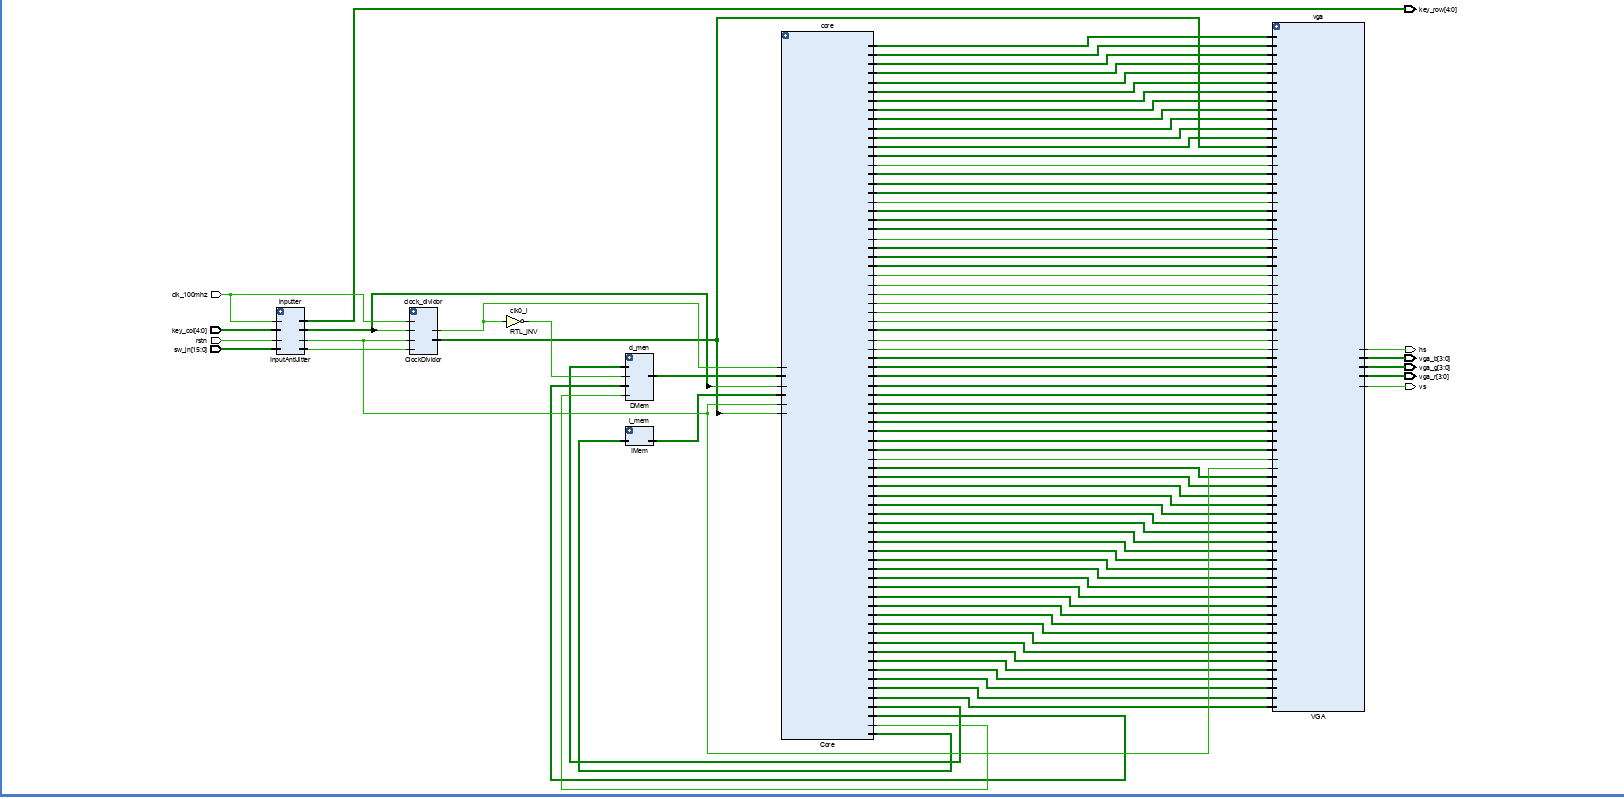
\includegraphics[width=1.0\textwidth]{yanzhen.png} %插入图片,[]中设置图片大小,{}中是图片文件名
%     \caption{验证结果图} %最终文档中希望显示的图片标题
%     \label{Fig.7} %用于文内引用的标签
% \end{figure}
\subparagraph{生成二进制文件} 选择左侧面板的Generate Bitstream或者点击上上的绿色二进制标志。同时生成Bitstream前要确保:之前已经综合、实现过最新的代码。如没有,直接运行会默认从综合、实现开始。此过程还要注意生成的bit文件默认存放在.runs下相应的implementation文件夹中
\subparagraph{烧写上板} 点击左侧的Open Hardware Manager $\rightarrow$ 点击Open Target $\rightarrow$ Auto Connect $\rightarrow$ 点击Program Device $\rightarrow$ 选择bistream路径,烧写。验证结果见实验结果部分。
